\section{Overview}
\subsection{The main results}
This paper is the second of a series on the mathematical structure of the Deep Linear Network (DLN). Our goal in these works is to shed new light on the training dynamics on deep learning through an analysis of the hidden symmetries of the DLN. This paper focuses on the concept of balancedness; we observe the natural role of Geometric Invariant Theory (GIT) in the DLN and use the Kempf-Ness theorems and related gradient flows to establish a new dynamic paradigm in deep learning. 

We summarize the essentials of the DLN below and refer to~\cite{MY-dln} for further context. The state space of the DLN consists of $N$ $d\times d$ matrices $\ww=(W_N,\ldots,W_1)\in \Md^N(\mathbb{F})$. The integers $N$ and $d$ are termed the depth and width respectively. The field $\mathbb{F}$ may be either $\mathbb{R}$ or $\mathbb{C}$ and we use $^*$ to denote the transpose or conjugate transpose respectively. The cost function $E$ for the DLN depends only on the end-to-end matrix 
\begin{equation}
    \label{eq:balanced-intro1}
    X= W_N W_{N-1} \ldots W_1.
\end{equation}
Training dynamics in the DLN is modeled by the gradient flow 
\begin{equation}
    \label{eq:balanced-intro1a}
    \dot{\mathbf{W}} = - \nabla_\mathbf{W}E(X(\mathbf{W})).
\end{equation}
The underlying Euclidean metric is described in Section~\ref{subsec:reg-flow} below.

%and a calculation with the chain rule reveals that equation~\eqref{eq:balanced-intro1} is equivalent to the system of equations
%\begin{equation}
%    \label{eq:balanced-intro2a}
%    \dot{W}_k = - (W_N\cdots W_{k+1})^* E'(X) (W_{k-1}\cdots W_{1})^*, \quad 1 \leq k \leq N,
%\end{equation}
%where $E'(X)$ is the matrix with entries $\tfrac{\partial E}{\partial $

The natural geometry of equation~\eqref{eq:balanced-intro1a} is that of a gradient flow on a fibered space. It is this aspect that we study in detail. Our results in this paper rely on the interplay between two complementary foliations of $\Md^N$: 
\begin{enumerate}
    \item The 
fibers $\fiberX$ of $\Md^N$ defined as the solution set to the polynomial equation~\eqref{eq:balanced-intro1} for each $X \in \Md$. 
\item the balanced variety 
$\balance_0$ defined as the solution set to the quadratic system 
\begin{equation}
    \label{eq:balanced-intro2}
     W_kW_k^* = W_{k+1}^*W_{k+1}, \quad 1\leq k \leq N-1.
\end{equation}
\end{enumerate}
The balanced variety is invariant under the gradient flow~\eqref{eq:balanced-intro1a} and has several fundamental properties (see~\cite[Thms. 2-8]{MY-dln})). It is foliated by rank into a collection of manifolds. When $X$ has full rank, it lies on a leaf of $\balance_0$, termed the balanced manifold $\balance$. We assume throughout this paper that $X$ has full rank in order to illustrate the new ideas without technical complications. The fibers and balanced manifold are illustrated schematically in Figure~\ref{fig:dln}.




%This result contrasts two different geometric structures: the fibers and the balanced varieties. The fiber $\fiberX$ over an end-to-end matrix $X$ is the algebraic variety defined by the polynomial equation
%\begin{equation}
%    \label{eq:balanced-intro1}
%    X= W_N W_{N-1} \ldots W_1.
%\end{equation}
%The balanced variety $\balance_0$ consists of matrices $\ww=(W_N,\ldots,W_1)\in \Md^N(\mathbb{F})$ such that 

We establish a minimum principle for balancedness that reveals a `hidden convexity' in deep learning. By hidden convexity we mean that the balanced manifold can be characterized by a class of minimum principles of which the following is the simplest. Consider the $L^2$ (ridge) regularizer 
\begin{equation}
    \label{eq:ridge}
    \|\ww\|_2^2 := \sum_{k=1}^N \Tr (W_k^* W_k).
\end{equation}

\begin{theorem}
\label{thm:intro} Assume $X$ has full rank. Then
\begin{equation}
\label{eq:variation1} \argmin_{\ww \in \fiberX} \|\ww\|_2 = \fiberX \cap \balance.
\end{equation}   
\end{theorem}
In what follows, we provide several interpretations and extensions of this theorem. The most important in practice is model reduction: Theorem~\ref{thm:intro} selects the simplest parametric description of a given end-to-end matrix $X$ (Section~\ref{subsec:occam}).  Our ideas on balancing are closely tied to linear systems theory; we show that both areas may be unified through the use of GIT (Sections~\ref{subsec:ls}--\ref{subsec:GIT}). In order to implement this idea in practice, we introduce a broader class of minimization principles along with new gradient flows ({\em regularizing flows\/}) with rigorous convergence guarantees (Section~\ref{subsec:reg-flow}). Finally, we use GIT to relate the DLN to mathematical physics and the Yang-Mills theory. Let us now explain these ideas in greater detail.

%\begin{remark}
%We have assumed that $X$ has full rank only for simplicity of statement. Theorem~\ref{thm:intro} is a consequence of the Kempf-Ness theorem, which characterizes the closure of $\fiberX$ in terms of norm minimization. We discuss the Kempf-Ness theorem and the hypotheses on $\fiberX$ more carefully in Section~\ref{sec:proofs}. 
%\end{remark}
%For now, we note that $\fiberX$ is always closed when $X$ has full rank. More generally, when $X$ has rank $r<d$, the condition 
%\begin{equation}
%    \label{eq:rank-condition} \mathrm{rank}(W_p)= \mathrm{rank}(W_{p+1}) = \mathrm{rank}(W_{p+1}W_p), \quad 1\leq p \leq N,
%\end{equation}
%for all $\ww \in \fiberX$ is equivalent to closure of $\fiberX$. 
\subsection{Balancedness, regularization and Occam's razor}
\label{subsec:occam}
%Theorem~\ref{thm:intro} relates balancedness to model reduction in the following way. The fiber $\fiberX$ consists of all parametrizations $\ww$ such that $W_N\cdots W_1 =X$. Theorem~\ref{thm:intro} asserts that a special subset of parameters, $\orbitx \subset \balance$, is selected by minimizing the $L^2$ regularizer. 
Theorem~\ref{thm:intro} is a form of Occam's razor. This is seen as follows.


Let $X = Q_N\Sigma Q_0^*$ denote the SVD of $X$. We define the {\em center\/} of $\fiberX$ to be the point $\bfC= (Q_N\Lambda,\ldots,\Lambda Q_0^*)$, with $\Lambda=\Sigma^{1/N}$.  Every point on $\fiberX$ may be obtained by translating the center through a group action. 

Given $N-1$ invertible matrices, $\mathbf{A}=(A_{N-1},A_{N-2},\ldots, A_1)$, we define the $\GLdC^{N-1}$ action 
\begin{equation}
    \label{eq:group-action1}
    \mathbf{A}\cdot \ww = (W_N A_{N-1}^{-1}, A_{N-1}W_{N-1}A_{N-2}^{-1}, \cdots, A_1 W_1).
\end{equation}               
This group action leaves $\fiberX$ invariant. We show (Lemma~\ref{le:group-orbit}) that each point in $\fiberX$ is of the form $\mathbf{A}\cdot \bfC$ for some $\mathbf{A} \in \GLdC^{N-1}$. 

Similarly, $\fiberX \cap \balance:=\orbitx$  is a $U_d^{N-1}$ group orbit, where $U_d$ is the unitary group. Each $\ww \in\orbitx$ is obtained by the group action $\bfQ\cdot \bfC$ where $\bfQ=(Q_{N-1},\ldots,Q_1)\in U_d^{N-1}$ (this is an easy modification of~\cite[\S 4]{MY-dln}).

The unitary orbit $\orbitx$ consists of the simplest parametric representations of $X$ amongst all admissible parametrizations $\ww \in \fiberX$. Certainly $\bfC= (Q_N \Lambda,\ldots,\Lambda Q_0^*)$ is a point in $\fiberX$ that contains no superfluous information: it depends on $X$ and $X$ alone. Further, since  
\begin{equation}
    \label{eq:group-action2}
    \|\ww\|_2 = \|\bfQ \cdot \ww\|_2, \quad \bfQ \in U_d^{N-1},
\end{equation} 
the minimizing set of $\|\ww\|_2$ must be invariant under  the $U_d^{N-1}$ action. 

Thus, Theorem~\ref{thm:intro} tells us that minimizing the $L^2$ regularizer, conditional on the end-to-end matrix $X$, yields the simplest parametric representations of $X$. It is in this sense that regularization in the DLN acts as a form of Occam's razor. 

\subsection{Balancedness in deep learning and linear systems theory}
\label{subsec:ls}
The concept of balancedness has arisen independently in linear systems theory and deep learning. Our main insight is that these concepts may be unified, allowing us to transport techniques used in linear systems theory to the DLN. In particular, we follow the work of Helmke to prove Theorem~\ref{thm:intro}~\cite{Helmke}. We augment his work with an analysis of the Riemannian geometry of $\fiberX$ and a rigorous analysis of balancing flows, providing an independent proof of Theorem~\ref{thm:intro}.

\subsubsection{Linear systems theory\/} 
The concept of balancedness arises in linear systems theory as follows. We consider the linear system
\begin{equation}
    \label{eq:ls1}
    \dot{x} = A x + B u, \quad y = Cx,
\end{equation}
where $x \in \C^n$ is the state, $u \in \C^m$ is the control, $y\in \C^p$ is the observation, and $A$, $B$ and $C$ are time-independent matrices with the appropriate dimensions. The input-output relation for this system is a relationship between the functions $u(t)$ and $y(t)$, $t \in [0,\infty)$, mediated by the equation~\eqref{eq:ls1}. It may be studied in the frequency domain through the Hankel matrix 
\begin{equation}
    \label{eq:ls2} H(z) = C (zI - A)^{-1}B, \quad z \in \C.
\end{equation}
Since $H(z)$ is unchanged under the action
\begin{equation}
    \label{eq:ls3}
    (A,B,C) \mapsto (MAM^{-1}, MB, CM^{-1}), \quad M \in \GLn,
\end{equation}
the class of triples ${(A,B,C)}$ whose Hankel matrix is $H(z)$ is a $\GLnC$ orbit.
Each choice $(A,B,C)$ that satisfies~\eqref{eq:ls2} is a realization of a linear system (the model) that is consistent with the input-output relation (the data). This notion dates to the work of Kalman~\cite{Kalman-real}. 

Model reduction in this context is the choice of an optimal realization consistent with the data. Norm balanced realizations minimize the Frobenius norm $\|MAM^{-1}\|_2^2 + \|MB\|_2^2 + \|CM^{-1}\|_2^2$ over $M \in \GLnC$. They constitute a principled choice of an optimal realization and have several favorable properties~\cite{Helmke}. This concept continues to be of great importance in Structured State Space Model (SSM) architectures, which are principled alternative to transformer architectures for modeling long sequences~\cite{Gu1}. In particular, the analysis of implicit bias in SSMs in analogy with implicit bias in the DLN is of current importance~\cite{Cohen-Karlik1,Cohen-Karlik2}.



\subsubsection{Balancedness in deep learning.\/} 
The concept of balancedness for the DLN was introduced by Arora, Cohen and Hazan in~\cite{ACH}. The underlying heuristic that `load is equally distributed across a balanced network' was formalized by Du, Hu and Lee for fully connected feed-forward networks with a homogeneous nonlinearity~\cite[Theorem 2.1]{JasonLee}. In our notation, this is the observation that when $\ww \in \balance$, then $\|W_k\|_2^2$ is independent of $k$. However, for the DLN, more is true. The singular values and singular vectors are aligned across the network: the SVD of $W_k = U_k \Lambda_k V_k^*$ and $W_{k+1}$ are related through $\Lambda_k=\Sigma^{1/N}$ for all $k$ and $V_k=U_{k+1}$ for $1\leq k \leq N-1$. This notion of alignment was examined by Ji and Telgarsky in several instances~\cite{Telgarsky}. The relationship between balancing and regularization appears also in the work of Soltanolkotabi, St{\"o}ger, and Xie (for $N=2$ and $W_2=W_1^*)$~\cite{SSX}. 

The surprising appearance of the conservation laws for the DLN (the moments $\bfG$ defined in equation~\eqref{eq:def-G} below) has also attracted attention. In several recent papers, Marcotte, Gribonval and Peyr\'{e}\/ have studied the relation between the symmetries and conservation laws for various neural networks~\cite{Peyre1,Peyre2,Peyre3}. Minimum principles for balancing weights, including an algorithm for balancing, have been introduced by Saul~\cite{Saul}. This work draws connections between symmetry in deep learning and mathematical physics in a manner that is similar in spirit to our work. Several other recent works have investigated equivariance and symmetry in deep learning~\cite{Kunin1,Tanaka-Kunin,Walters}. Finally, we note that the interplay between minimum principles and flatness has been studied by Ding, Drusvyatskiy, Fazel and Harchaoui~\cite{DDFH} and that a stratification of the loss landscape for the quadratic loss function has been studied by Achour, Malgouyres and Gerchinovitz~\cite{Achour}.

Our work does not rely on the techniques in the above papers though it builds on these themes. Instead, our work is closest in spirit to the relationship between optimization problems and integrable gradient flows on adjoint orbits studied by Bloch, Brockett and collaborators in the 1990s~\cite{Bloch1994,BBR}. Recent developments in this vein have extended these geometric principles to high-dimensional machine learning and quantum control, reinforcing the notion that the training dynamics of deep architectures are fundamentally governed by the underlying Riemannian geometry and conservation laws induced by parameter space symmetries~\cite{wang2024dynamical}.

%We develop this approach for the DLN, providing a rigorous variational principle based on well-founded geometric principles that characterizes the relationship between regularization and learning in the DLN. We see the DLN as a benchmark model that provides insight into the harder challenges of nonlinear networks.


\subsection{GIT, the moment map and duality}
\label{subsec:GIT}
The main goal in Geometric Invariant Theory (GIT) is to classify the orbit space of a group acting on a vector space~\cite{Mumford-Fogarty}. We do not study the orbit space of the DLN in full generality. However, we note some important consequences of the general theory.


%A powerful consequence of the Kempf-Ness technique is that the orbit space may be equipped with a symplectic geometry using the Marsden-Weinstein reduction \color{blue} (see. e.g. \cite{??}). \color{red}[Can we put in some standard reference for folks who haven't encountered the Marsden-Weinstein reduction?] \color{black} 

\subsubsection{The moment map}
Define the $N-1$ Hermitian matrices
\begin{equation}
    \label{eq:def-G} G_k = W_kW_k^* - W_{k+1}^*W_{k+1}, \quad 1\leq k \leq N-1.
\end{equation}
The Hermitian matrices $\{G_k\}_{k=1}^N$ are conserved under the gradient flow of an arbitrary loss function $E$~\cite[Theorem 2]{MY-dln}. The appearance of such a large number of conservation laws for a {\em gradient\/} flow is surprising at first sight. Indeed, we expect conservation laws for {\em Hamiltonian\/} systems, not gradient flows!   

The Kempf-Ness theorem explains this phenomena. The $\{G_k\}_{k=1}^{N-1}$ are obtained from the moment map corresponding to the invariance of $\tfrac{1}{2}\|\ww\|_2^2$ under the action
\begin{equation}
    \label{eq:moment1} \ww \mapsto \mathbf{U}\cdot \ww : = (W_N U_{N-1}^*,U_{N-1} W_{N-1} U_{N-2}^*,\cdots, U_1 W_1),
\end{equation} 
for $\mathbf{U}=(U_{N-1},\ldots, U_1) \in U_d^{N-1}$. The moment map is simply
\begin{equation}
    \label{eq:moment2}
    \MdC^N \to \Her_d^{N-1}, \quad \ww \mapsto \mathbf{G}:=(G_{N-1},\cdots,G_1).
\end{equation}
We explain how these arise in Section~\ref{sec:kempf-ness}. Loosely speaking, the moments $\mathbf{G}\in \Her_d^{N-1}$ may be seen as the analogues in deep learning of dual variables in the study of conic programs. 
%The factor of $2$ in~\eqref{eq:moment2} arises because we use the normalization convention in~\cite{Ness} for the moment map.

%The factor of $2$ is due to normalization (the moment map associated to $\|\ww\|_2^2/2$ is $\bfG$).

\subsubsection{Summary}
In terms of mathematical structure, the variational formulation of balancedness in linear systems theory and the DLN reduces to the minimization of a unitarily invariant squared norm on a group orbit. This problem has been solved by the Kempf-Ness theorem in GIT~\cite{Kempf}. Thus, balancedness theorems in both fields are consequences of the Kempf-Ness theorem. However, the Kempf-Ness theory does not provide quantitative rates of convergence or practical balancing algorithms. To this end, we use the Riemannian geometry of fibers to construct balancing flows with rigorous convergence guarantees (Theorem~\ref{thm:reg-flow} and Theorem~\ref{thm:ness-flow}). 


%In fact, GIT provides a powerful new toolbox for deep learning as discussed below.

This unification also allows us to reflect on common themes in the conceptual foundations of deep learning and linear systems theory. As Kalman writes in~\cite{Kalman-can}, a dynamical system may be described in two distinct ways: (i) by means of state variables (a model such as Newton's laws or equation~\eqref{eq:ls1}) and (ii) by input-output relations (a black box whose inner workings are opaque to the user but produces data such as $H(z)$). For the vast number of users of deep learning, it is the input-output relation that matters. However, for designers of the architecture of neural networks and for a complete scientific understanding of deep learning, it is necessary to understand training dynamics from first principles.



%\color{red}[Somewhere, maybe here, we should add a sentence citing some of the ML papers where balancedness has arisen. (Need to do literature search; recording a few links in commented text here)] 

%https://proceedings.neurips.cc/paper_files/paper/2018/file/fe131d7f5a6b38b23cc967316c13dae2-Paper.pdf
%https://openreview.net/pdf?id=HJflg30qKX&utm
%https://arxiv.org/pdf/1810.02281
%\color{black}

Our main finding then is that in both deep learning and linear systems theory, balanced (manifolds and realizations) correspond to optimal descriptions of the input-output relations in terms of the parameters of the model. 


%\begin{remark}
%\label{rem:duality}

%\end{remark}

\subsection{Regularizing flows and the learning flow}
\label{subsec:reg-flow}
Recall that the state space for a gradient flow is a Riemannian manifold. Thus, in order to define gradient flows on $\fiberX$ and $\balance$, we must equip them with a Riemannian metric. 

It is only the complex case that requires some comment. When $\mathbb{F}=\C$, we equip $\Md(\C)$ with the inner-product
\begin{equation}
    \label{eq:ipc-1}
    \langle A,B  \rangle =  \mathrm{Re}\,\Tr \left( A^* B\right).
\end{equation}
Writing $A=a+ib$ and $B=c+id$ for the real and imaginary parts, we see that 
\begin{equation}
    \label{eq:ipc-2}
    \langle A, B \rangle =  \Tr \left( a^Tc+ b^Td\right),
\end{equation}
so that $\Md(\C)$ has the same norm as the real vector space $\Md(\R)\times \Md(\R)$. Similarly, we define the norm on $\Md^N(\C)$
\begin{equation}
    \label{eq:ipc}
    \langle \mathbf{A}, \mathbf{B} \rangle = \sum_{k=1}^N \mathrm{Re}\,\Tr \left( A_k^* B\right).
\end{equation}
This inner-product defines $\Md^N(\C)$ as a Euclidean space. Since the fiber $\fiberX$ and the balanced variety $\balance$ are defined as the solutions to the algebraic equations~\eqref{eq:balanced-intro1} and~\eqref{eq:balanced-intro1}, they are embedded Riemannian manifolds of the Euclidean space $\Md^N(\mathbb{F})$ under natural assumptions on $X$ (for example, when $X$ has full rank). We denote the resulting Riemannian manifolds $(\fiberX,\iota)$ and $(\balance,\iota)$ respectively. 

%When the matrices are real, it is clear that both $\fiberX$ and $\balance$ are smooth embedded submanifolds of $\Md$ under natural assumptions on $X$ (for example, when $X$ has full rank). Thus, they inherit the Euclidean metric from $\Md$. 

We study two complementary gradient flows on these manifolds:
\begin{enumerate}  
\item {\em Regularizing flows}: This is the gradient flow of a regularizer $R(\ww)$ on the Riemannian manifold $(\fiberX,\iota)$. Theorem~\ref{thm:intro} corresponds to the regularizer $R(\ww)= \tfrac{1}{2}\|\ww\|_2^2$ and the gradient flow
\begin{equation}
\label{eq:reg-gradient1}
    \dot{\mathbf{W}}= -\frac{1}{2}\mathrm{grad}\,\|\mathbf{W}\|_2^2, \quad \mathbf{W}\in (\fiberX,\iota).
\end{equation}
We also consider the gradient flow of the squared moment map, $R(\ww)= \tfrac{1}{2}\|\bfG\|^2$ (see Remark~\ref{rem:ness-flow} below). Theorem~\ref{thm:intro} extends to include the Schatten $p$-norms as regularizers for $1<p<\infty$. It does not yet include the important case $p=1$ (see Theorem~\ref{thm:intro-revised} in Section~\ref{sec:kempf-ness}). 
\item {\em The learning flow}: This is the gradient flow of the loss function $E(X)$ on $(\balance,\iota)$
\begin{equation}
\label{eq:learn-gradient1}
    \dot{\mathbf{W}}= -\mathrm{grad} \,E(X(\ww)), \quad \ww\in (\balance,\iota).
\end{equation}
\end{enumerate}
We show that the regularizing flow for the $L^2$-regularizer is exactly solvable in the following sense. 
\begin{theorem}
\label{thm:reg-flow} Assume $X$ has full rank and $\ww(t)$ solves equation~\eqref{eq:reg-gradient1} with initial condition $\ww_0 \in \fiberX$. Then the moments $\mathbf{G}(t)$ satisfy
\begin{equation}
    \label{eq:reg-gradient2}
    \mathbf{G}(t) = \mathbf{G}_0 e^{-2t}, \quad t \geq 0.
\end{equation}
\end{theorem}
Thus, the moment map $\ww \mapsto \mathbf{G}$ reduces the regularizing flow to scaling at a uniform rate. Since the balanced variety is the inverse image $\mathbf{G}^{-1}\{\mathbf{0}\}$, Theorem~\ref{thm:reg-flow} establishes attraction to the balanced manifold at a constant rate. 
\begin{remark}
\label{rem:ind-proof}
The methods that underly Theorem~\ref{thm:intro} and Theorem~\ref{thm:reg-flow} are different. Theorem~\ref{thm:intro} is an application of the Kempf-Ness theorem and thus relies on ideas primarily from algebraic geometry. On the other hand, Theorem~\ref{thm:reg-flow} relies on explicit matrix computations that reflect the underlying Riemannian geometry. 
\end{remark}
\begin{remark}
\label{rem:low-rank-scaling}
The assumption on rank may be relaxed in both Theorem~\ref{thm:intro} and Theorem~\ref{thm:reg-flow}. Theorem~\ref{thm:intro} requires that we work with group orbits so that we may apply the Kempf-Ness theorem. On the other hand, Theorem~\ref{thm:reg-flow} requires only that we work on a Riemannian manifold (in particular, the calculations in Section~\ref{sec:reg-flow} may be generalized to the setting of rank $r<d$). When $X$ has full rank, both these conditions are true. We focus on this situation so that our calculations are most transparent.

The underlying algebraic geometry, including the foliation by rank, has been analyzed in generality by Shewchuk and Bhattacharya~\cite{Shewchuk} and Pepin Lehalleur and Rim\'{a}nyi~\cite{Lehalleur}. While these results parallel one another, the methods are different: the article~\cite{Shewchuk} emphasizes linear algebra, whereas~\cite{Lehalleur} organizes these calculations using the language of quiver representations. The relationship between these geometric structures and the loss landscape for the quadratic loss function is a topic of current interest.
\end{remark}



\begin{remark}
\label{rem:learn-flow}
The learning flow~\eqref{eq:learn-gradient1} on $(\balance,\iota)$ is equivalent to the gradient flow
\begin{equation}
    \label{eq:learning-flow} \dot{X} = - \mathrm{grad}_{g^N} E(X), \quad X \in (\Md,g^N).
\end{equation}
Here the Riemannian manifold $(\Md,g^N)$ is obtained by Riemannian submersion from $(\balance,\iota)$ through the map $\ww \mapsto X$. The metric may be described explicitly~\cite{GM-dln}.

This statement is a synthesis of results from~\cite{ACH,Bah,MY-dln,MY-RLE} that identifies the learning flow as an equilibrium thermodynamic  process.
\end{remark}

\begin{remark}
\label{rem:reg-flow}
Our regularizing flow~\eqref{eq:reg-gradient1} differs from what has been used in linear systems theory. Gradient flows on $\GLn$ that balance a triple $(A,B,C)$ (`balancing flows') have been studied by Helmke and Moore~\cite{Helmke-Moore}. These gradient flows were inspired by Brockett's double-bracket flow on $O_n$~
\cite{Brockett}. However, these works use the normal metric on $\GLn$ and $O_n$ respectively, not the induced metric $\iota$. In our view, it is necessary to use the induced metric instead because (i) this conforms to the Euclidean metric used in practice for deep learning; (ii) it allows us to include noise in a geometrically natural manner using Riemannian Langevin equations (cf. \S \ref{subsec:noise}). %Theorem~\ref{thm:reg-flow} shows that the regularizing flow is analytically and numerically tractable once one has adopted the correct viewpoint.
%We present the RLE related to~\eqref{eq:learning-flow} in the companion paper~\cite{MY-RLE}.
\end{remark}
\begin{remark}
\label{rem:ness-flow}
Kirwan and Ness studied the Morse theory of the squared moment map in their pioneering work on GIT~\cite{Kirwan,Ness}. Ness studied the related gradient flow~\cite[\S 3-7]{Ness} and analyzed its convergence properties. In our context, this regularizing flow, which we term the {\em Kirwan-Ness\/} flow, is given by~\footnote{The reader should note that we use a different normalization from Ness. We find it more convenient to use $\tfrac{1}{2}\|\mathbf{G}\|_2^2$ rather than $\|\mathbf{G}\|_2^2$.}
\begin{equation}
\label{eq:reg-gradient5}
    \dot{\mathbf{W}}= -\frac{1}{2}\mathrm{grad}\,\|\mathbf{G}\|_2^2, \quad \mathbf{W}\in (\fiberX,\iota).
\end{equation}
A striking feature of the DLN is that this flow is given explicitly by the cubic system
\begin{equation}
    \label{eq:ness-flow-coords}
    \dot{W}_k = 2(W_kG_{k-1}-G_{k}W_k), \quad 1\leq k \leq N,
\end{equation}
with the convention $G_N=G_0=0$. This allows us to adapt the general theory from GIT for the purpose of balancing in deep learning (see Section~\ref{sec:ness} below). 

The Kirwan-Ness flow also provides a technical relationship between deep learning and mathematical physics through the common structure of Yang-Mills theory as discussed in Uhlenbeck's recent work~\cite{Atiyah-Bott-YM,Uhlenbeck2026}. We note that mathematical physics techniques such as the renormalization group and diagrammatic expansions have been used to study deep learning, but rigorous mathematical justification of these ideas is still limited~\cite{Hanin-book}. 
%an excellent exposition is provided by Lerman~\cite{Lerman}.
%It is clear that the functional $\|\mathbf{G}\|_2^2$ is minimized on the balanced manifold. 
\end{remark}

\begin{figure}
    \centering
    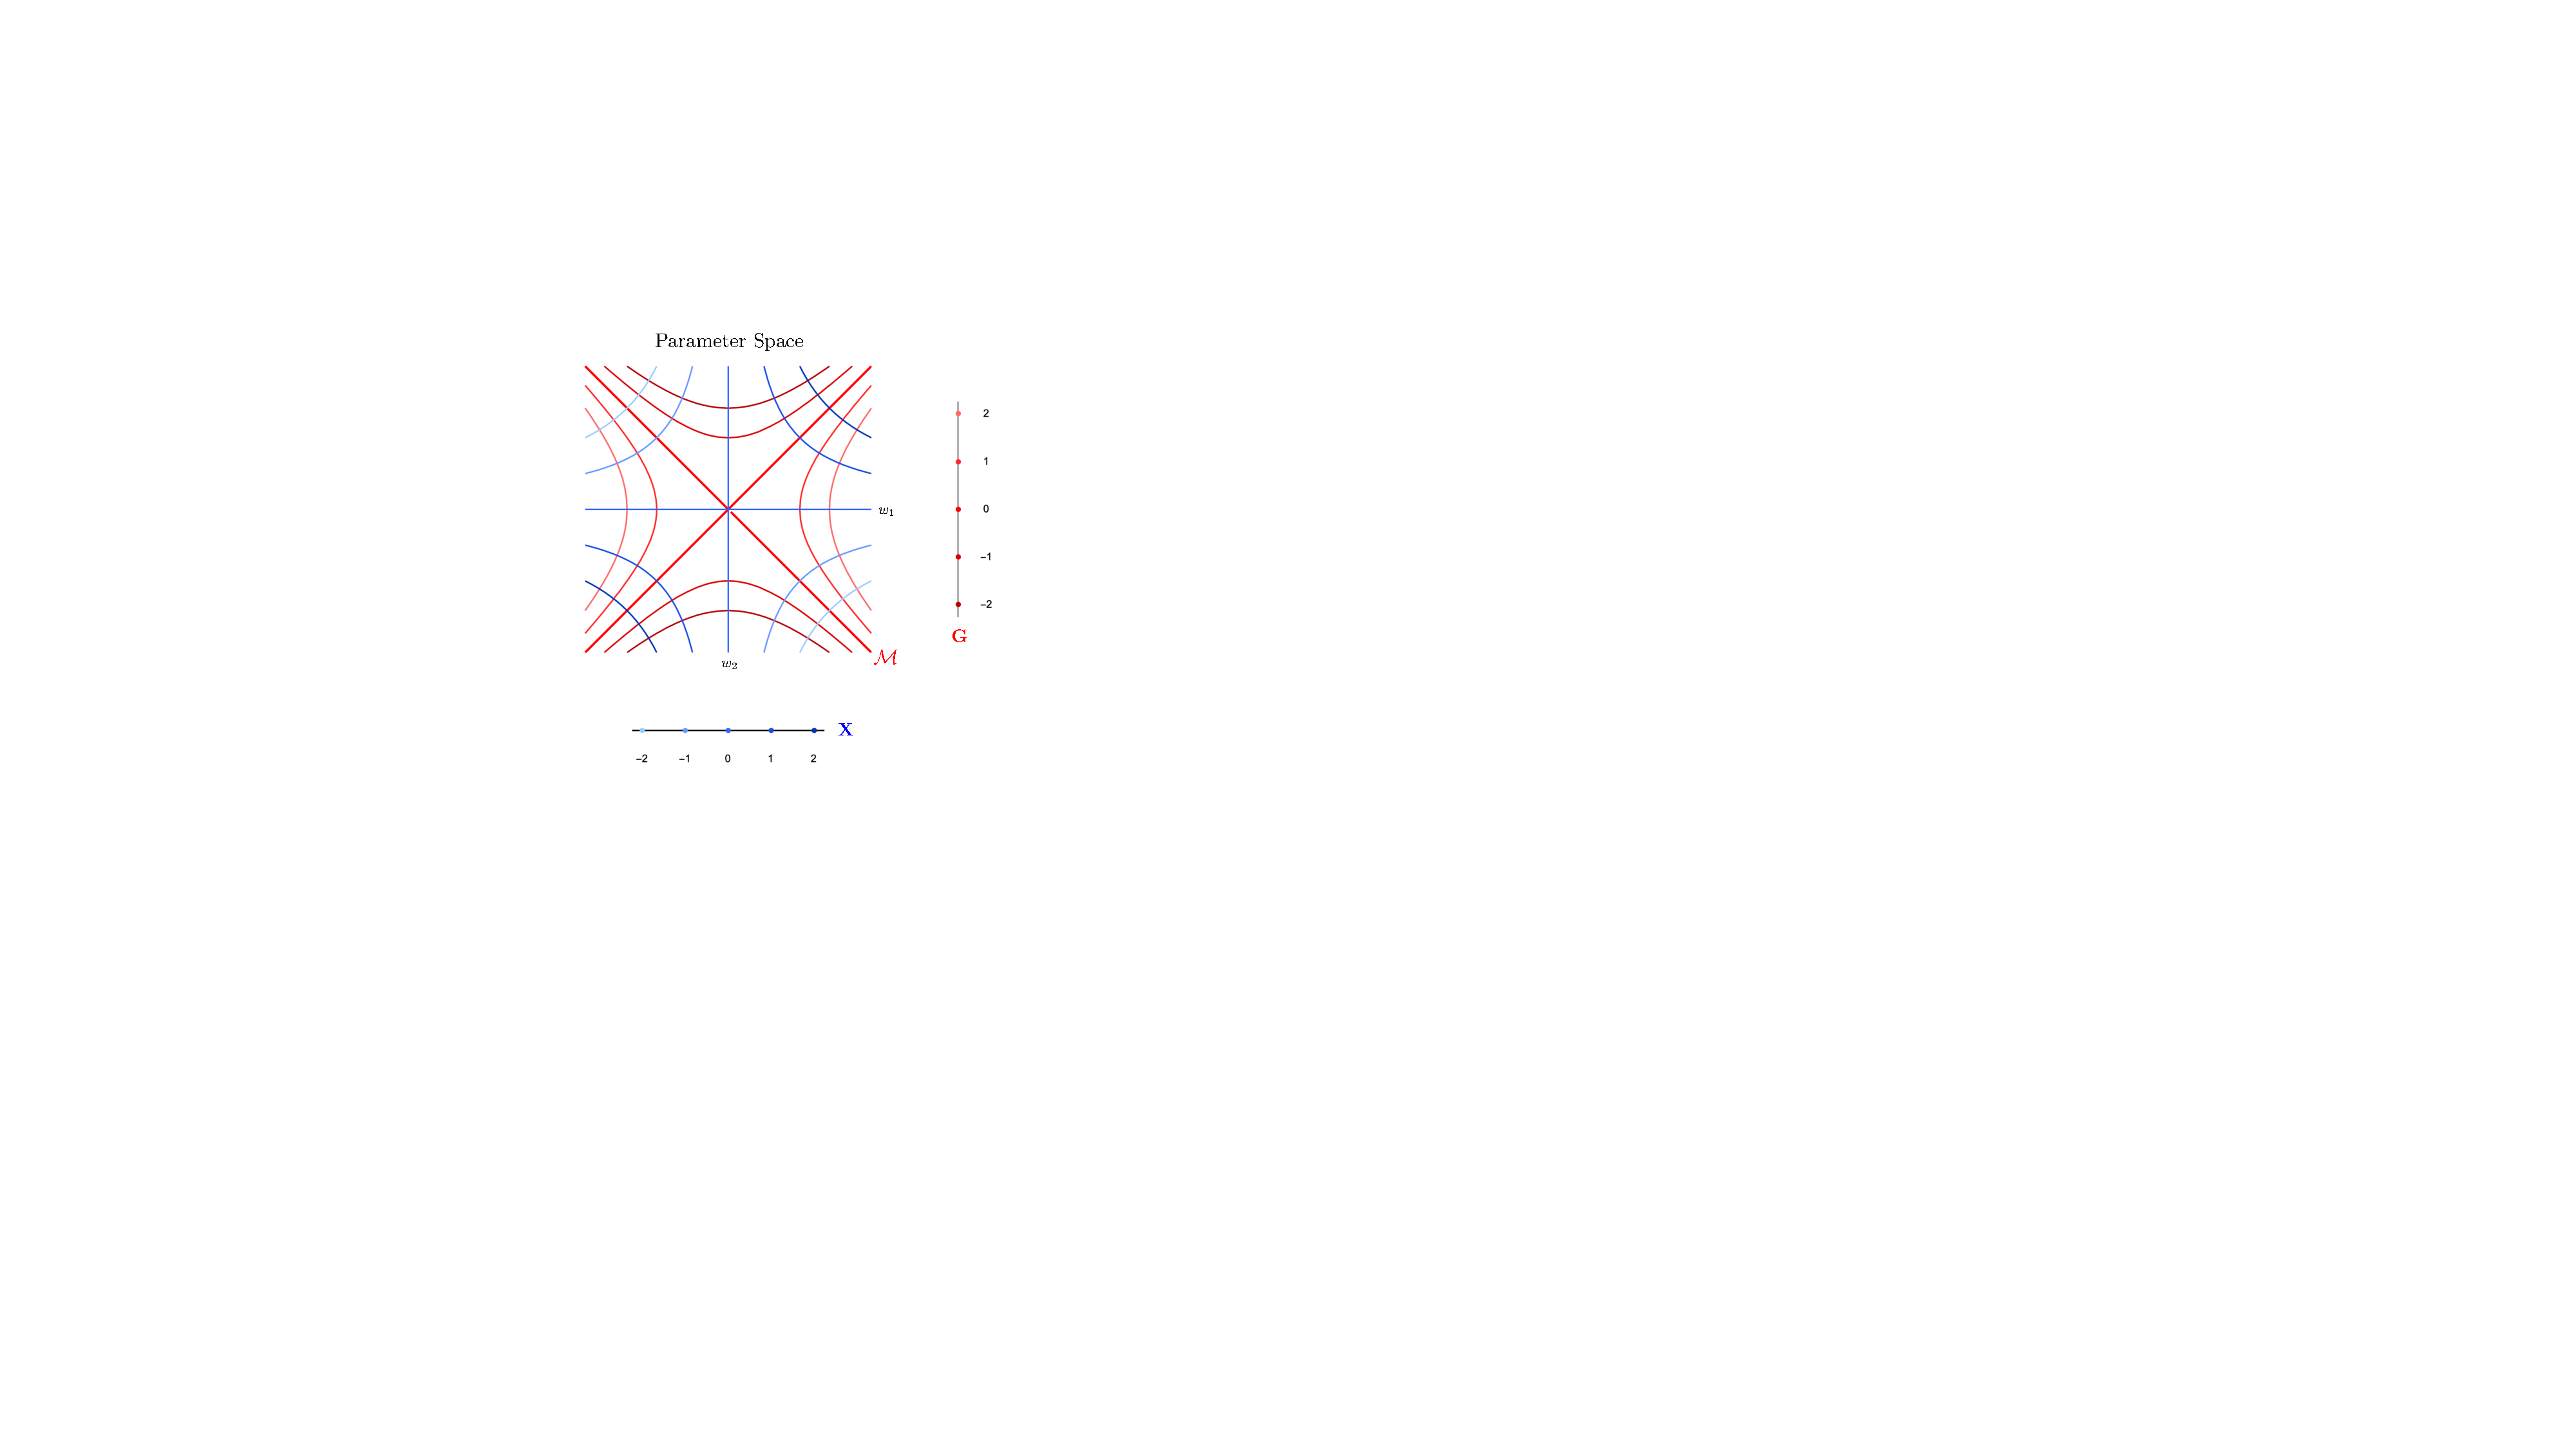
\includegraphics[trim={425 500 1200 225}, clip, width=.7\linewidth]{./figures/Fig1RevisedFinal.pdf}
    \caption{This figure describes the orthogonal foliation of $\Md^N$ by the balanced varieties $\balance_{\mathbf{G}}$ and fibers $\fiberX$ in the simplest case ($d=1$ and $N=2$ and real matrices). The regularizing flow lies on the hyperbola $w_2w_1=x$. The learning flow lives on the asymptotes $w_2 = \pm w_1$. It is intuitively clear that the minimizers of $|w|^2$ on the fiber $w_2w_1=x$ are the points $(\pm \sqrt{x},\pm \sqrt{x})$. Theorem~\ref{thm:intro} establishes the analogous property in general.}
    \label{fig:dln}
\end{figure}

\begin{figure}[h]
    \centering
    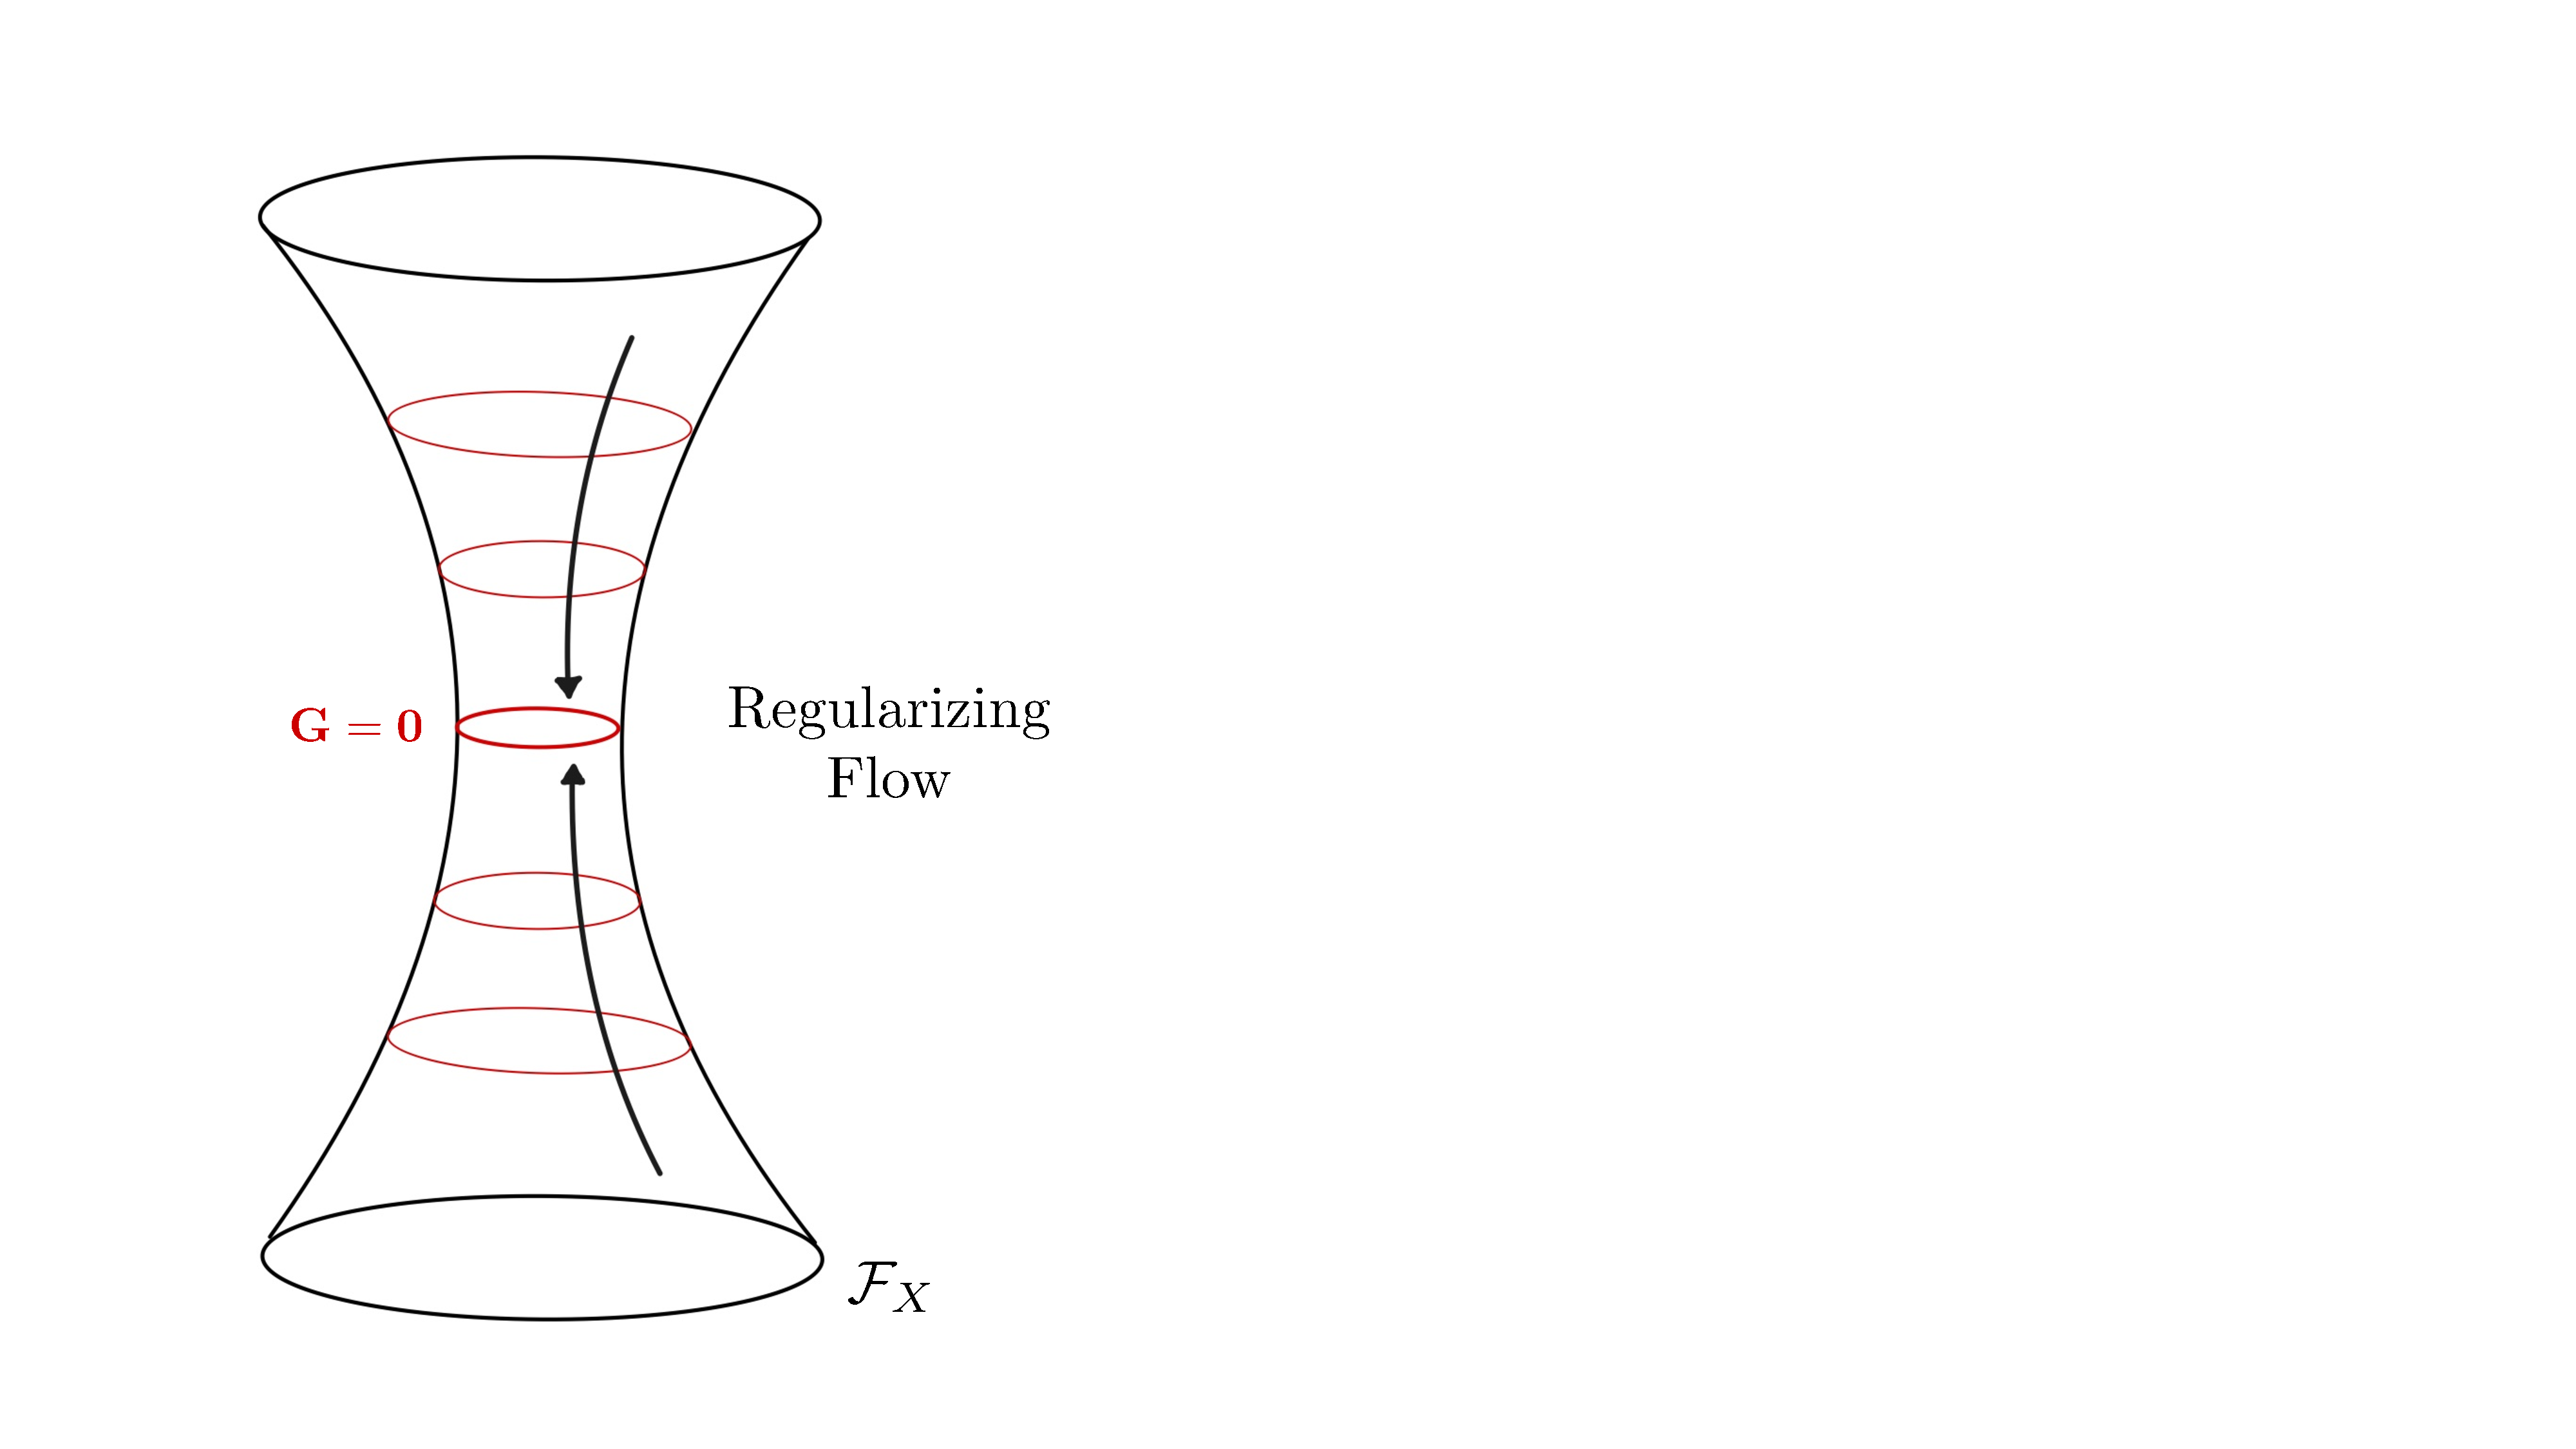
\includegraphics[trim={175 75 1100 75}, clip, width=.4\linewidth]{./figures/figure2Revised.pdf}
    \caption{The regularizing flow (see Theorem~\ref{thm:reg-flow}) on $\fiberX$. When $d\geq 2$ the fiber $\fiberX$ is sliced by the moments $\bfG$ into topologically equivalent components $\fiberX \cap \balance_\bfG$. The regularizing flow evolves the slices at a uniform exponential rate towards the minimizing orbit $\orbitx$ corresponding to $\bfG=\mathbf{0}$.}
    \label{fig:reg-flow}
\end{figure}


\begin{figure}[h]
    \centering
    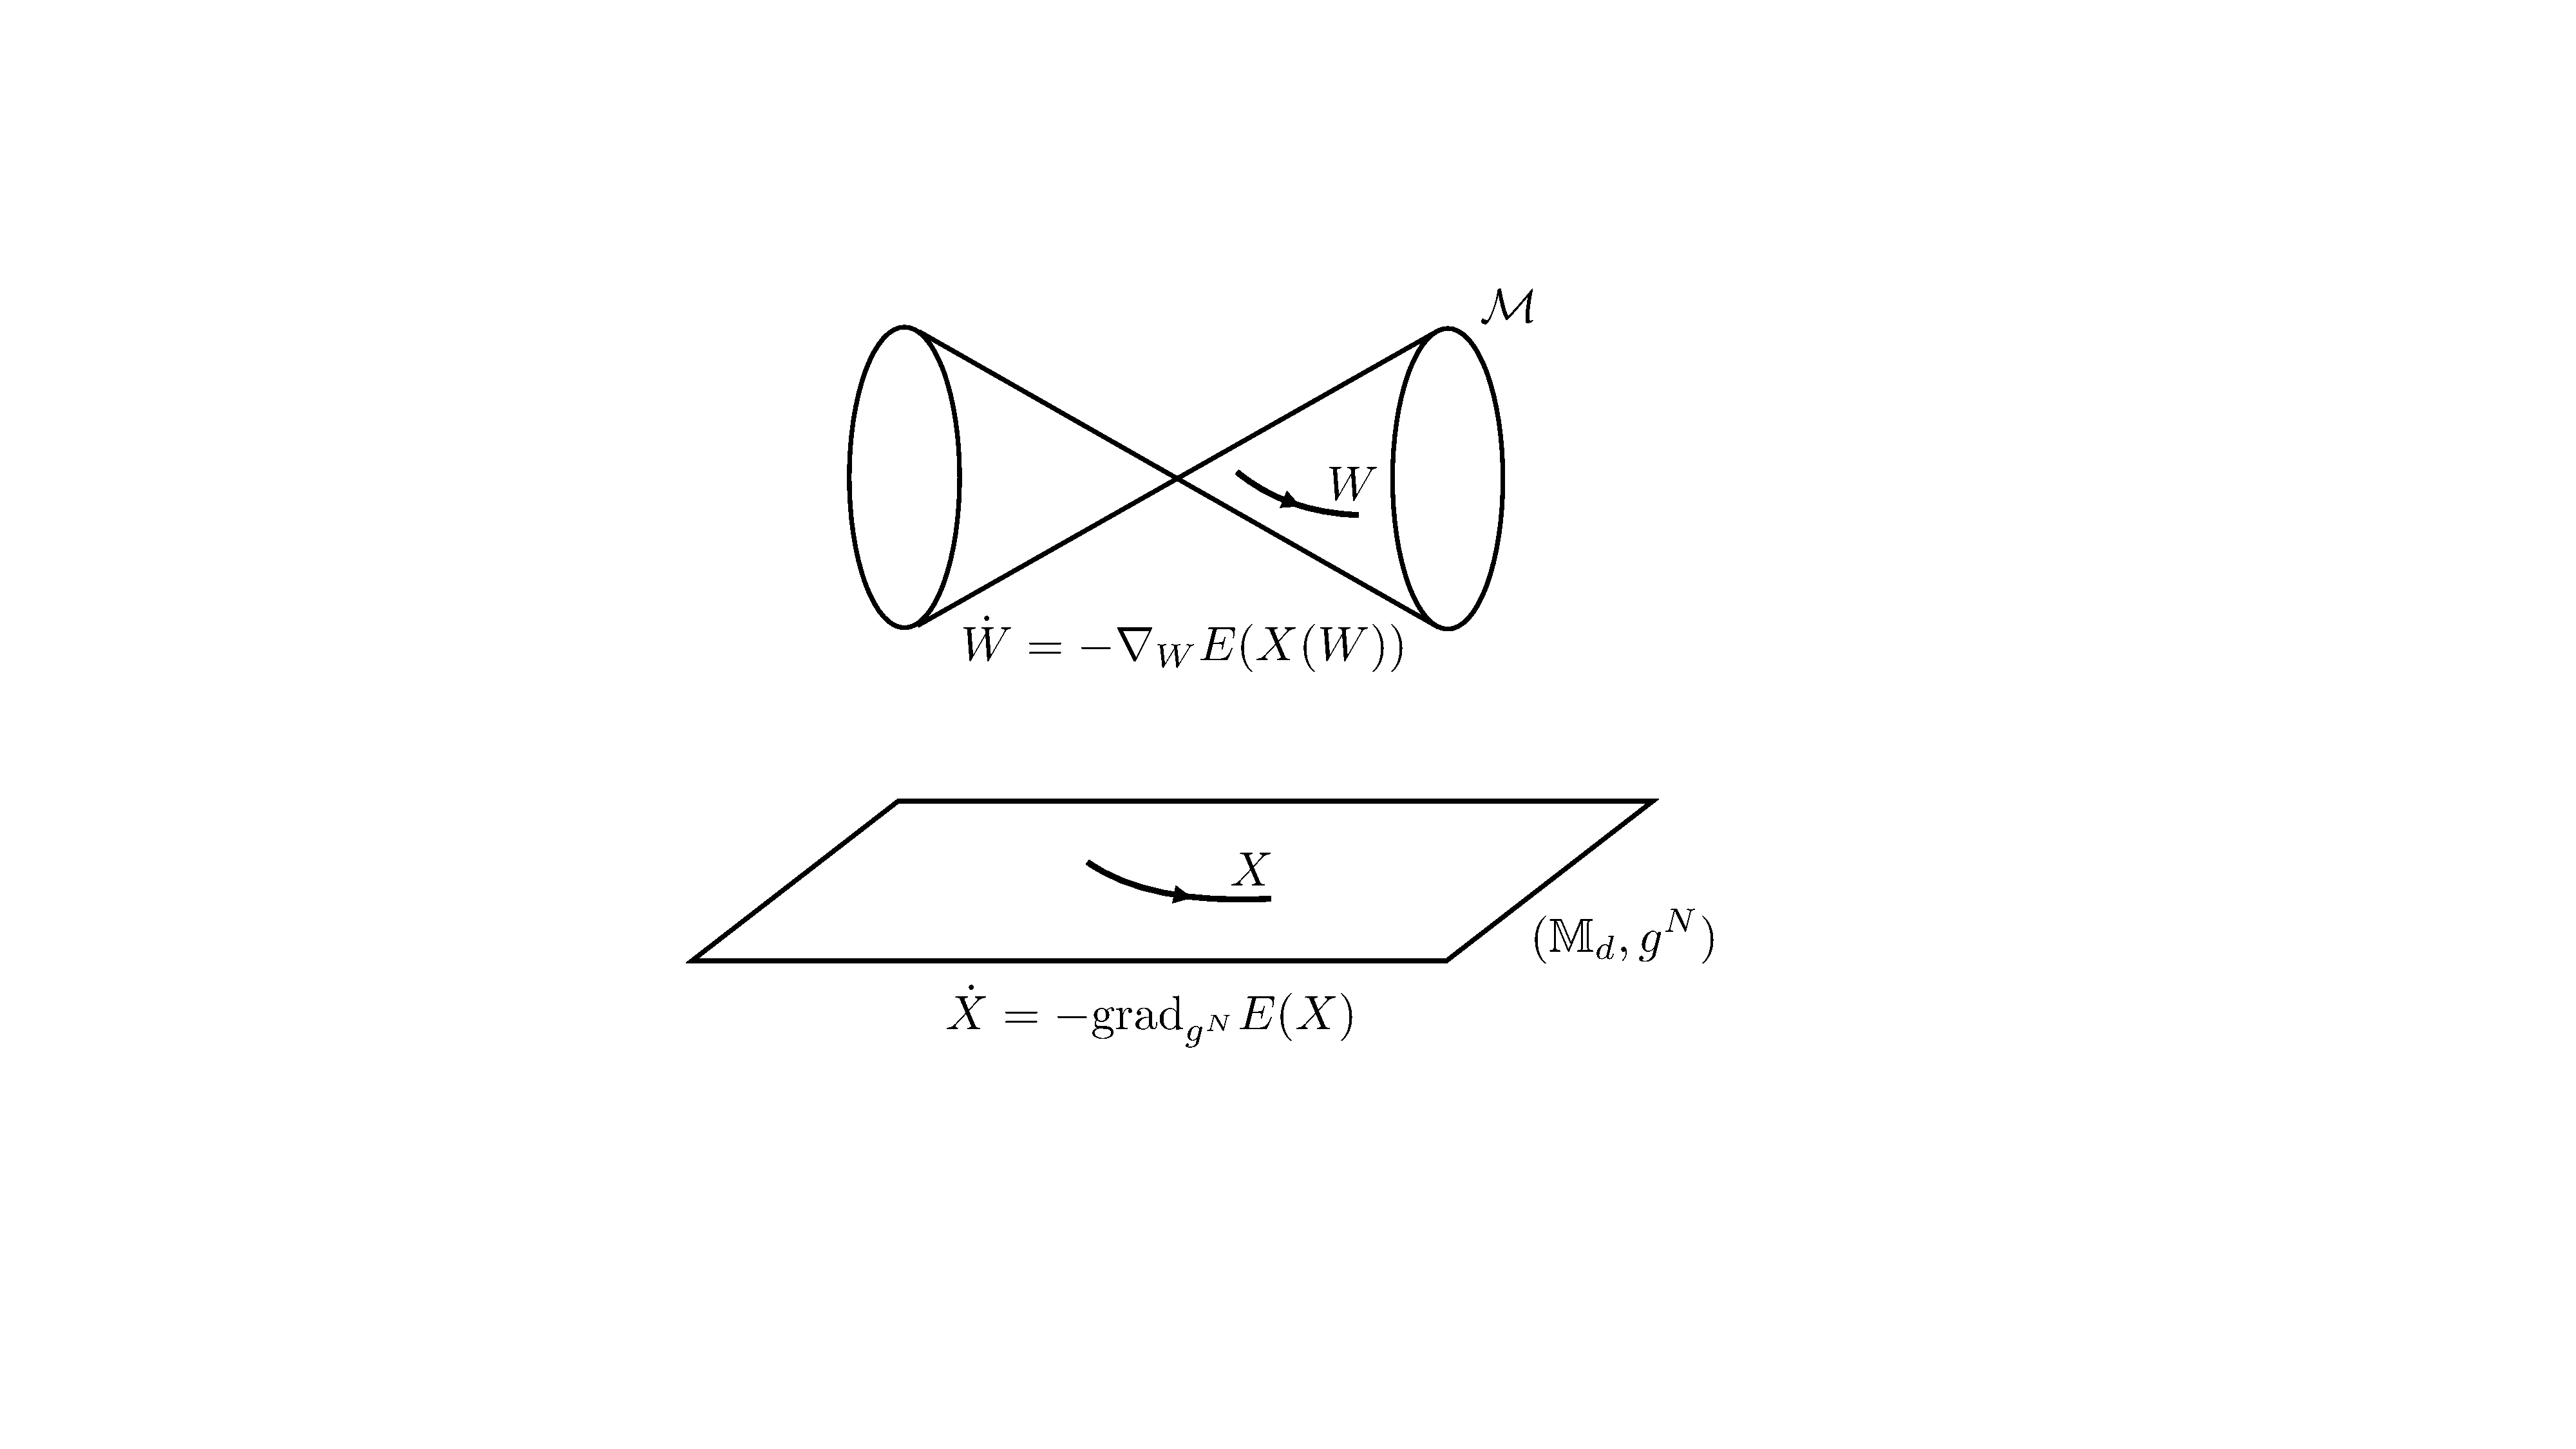
\includegraphics[trim={500 275 600 200}, clip, width=.6\linewidth]{./figures/figure3keynote.pdf}
    \caption{The learning flow. There are two equivalent descriptions: the balanced manifold $\balance$  is invariant under the gradient flow $\dot\ww =-\nabla_\ww E(X(\ww)$ of the cost function. Further, the dynamics of the end-to-end matrix $X$ are given by the Riemannian gradient flow $\dot{X}=-\grad_{g^N} E(X)$ on $(\Md,g^N)$ where the manifold $(\Md,g^N)$ is obtained by Riemannian submersion from $(\balance,\iota)$.}
    \label{fig:learn-flow}
\end{figure}


\subsection{Organization of the paper}
We first study the Riemannian geometry of fibers, introduce the regularizing flows and establish their convergence (Theorem~\ref{thm:reg-flow} and Theorem~\ref{thm:ness-flow}) in Section~\ref{sec:reg-flow}. This is followed by a discussion of the Kempf-Ness theorem, its generalization, the Azad-Loeb theorem, and the application of GIT to the DLN. The paper concludes with a discussion of a new dynamic paradigm suggested  by the methods of this paper.









